
\section{The Teacher Assistance Tools}
\label{sec:teach-assist-tools}

As discussed in the previous sections, MiGen’s Teacher Assistance (TA)
Tools aim to support the teacher in following students' progress on
tasks set for them to undertake in eXpresser, so that the teacher can
intervene with additional support for the class as a whole or for
individual students as appropriate, e.g. in providing additional
guidance, encouraging reflection, or setting new goals. Of course,
teachers are very well able to judge what constitutes progress and to
support their students by appropriate prompts and nudges. As we
discussed in Section 1, the problem for them is to do that effectively
with a whole class of students as students are working on exploratory
learning tasks using eXpresser all at the same time. MiGen's TA tools
aim to support teachers by reducing their cognitive load and
increasing their awareness of the classroom `state’.
 
We now give a more detailed description of each of the TA tools
introduced in Section 2. We refer the reader back to the figures in
that Section for visual illustrations of each tool. The most detailed
tool, and the one developed first chronologically, is the ST tool. So
we begin with a description of that below, followed by the CD tool and
finally the GA tool.

\subsection{Student Tracking}
\label{sec:student-tracking}

The Student Tracking tool keeps a track of all TI and TD indicators
generated by each student as they interact with the eXpresser. These
indicators are shown chronologically in a top-down timeline for each
student (see Figure 2), with one column for each student in the
class. Timelines can be made thinner or wider using a slider. Using
narrower timelines provides a general overview of all the students’
timelines but cannot show the text associated with the
indicators. Using wider timelines allows a more detailed exploration
of the indicators for a particular student. Timelines can also be made
shorter or longer (i.e. so that a vertical pixel represents a longer
or shorter time period). A shorter view allows the teacher to
undertake a general appraisal of all the students' actions so far. A
longer view allows the teacher to look in detail at their interaction
during a specific time period.
 
The indicators are displayed as horizontal bars or vertical lines
depending on whether they are event indicators or state
indicators. Event indicators relate to an action that happens at a
single time point, e.g. goal accomplished, pattern created, feedback
received. State indicators represent an aspect of the students'
interaction that is always monitored and has a value of `yes’, `no’ or
`maybe’.  Examples are `student is active’, `student is animating
their model’, and `a plausible building block is in use’. We refer the
reader to [IEEETLTPaper] for a detailed description of the different
categories of event and state indicators.

Referring back to Figure 2, we see that student CI began by trying to
animate her model, then placed some single tiles on the canvas, and
then created a pattern. This last line is shown in Red, indicating
that the pattern was not considered to be correct by the system for
the task at hand (so this is a Task Dependent indicator). Student CI
was then inactive for a while (shown by the `ACTIVE’ state indicator
turning from Green to Red). At this point the teacher may have
intervened, encouraging the student to place tiles to construct a
correct pattern. The system next detects `rhythm’ in the student’s
tile placements (as shown by the occurrence of the Blue feedback
indicator), in the sense that the tiles placed on the canvas match
part of the target model. The system displays a message to the
student: “It seems you keep repeating this building block. Why don’t
you use it to make a pattern?”. We finally see that the student
creates a correct pattern.
  
The identification of the full set of indicators was achieved through
an iterative process undertaken as a joint activity with our teacher
collaborators during Phases A and B of the project. This resulted in
the development of over 50 indicators being tracked by the
system. During the classroom trials in Phase B it became evident that
it was infeasible for teachers to comprehend all of this information
at one time within the ST tool. Larger combinations of the indicators
would be useful for after-class analysis, but the number of indicators
to be displayed during the classroom session needed to be reduced.

The ST tool was therefore extended to allow the teacher to select
which indicators should be shown or hidden, depending on the teacher’s
current needs. For convenience, the indicators are divided into a
number of `families’ which the teacher can select to be collectively
shown or hidden (the teacher can also select individual indicators to
be shown/hidden). The families of indicators are: event indicators,
state indicators, building-block related indicators, rule-related
indicators, and important indicators. This last category of 'important
indicators' was identified in consultation with a team of pedagogical
experts in Phase C of the project. These indicators are considered by
the pedagogical experts as being the most relevant for use during the
lesson. The default display of the current ST tool is with this family
of important indicators being shown and the rest of the indicators
being hidden.  The important indicators are all event indicators and
are the following:

\begin{itemize}
        	\item Number unlocked (i.e. variable created), – displayed in Green;
        	\item Correct local rule created (i.e. correct colour
              allocation in a pattern) – displayed in Green;
        	\item Incorrect local rule created (i.e. incorrect colour
              allocation in a pattern), – displayed in Red;
        	\item Correct global rule created (i.e. correct colour
              allocation for the whole model) – Green;
        	\item Incorrect global rule created (i.e. incorrect colour
              allocation for the whole model) – Red;
        	\item Plausible building-block made (i.e. probably leads
              to a correct solution of the task) – Green;
        	\item Implausible building-block made (i.e. will probably
              not lead to correct solution of task) – Red;
        	\item Pattern made using a plausible building-block – Green; 
        	\item Pattern made using an implausible building-block –
              Red;
        	\item General solution created and animated – Green, if
              the solution animates correctly, otherwise Red;
        	\item Goal checked by system (i.e. one of the task goals
              has been detected as being accomplished by the system) –
              Green;
        	\item Help requested by the student – Blue; 
        	\item Feedback shown to the student – Blue.
  \end{itemize}
 
Hovering with the cursor over one of the indicators in the ST display
provides further  information: the full name of the student, full name
of the indicator, and precise time it occurred. For some indicators
additional information is also shown, e.g. for the indicator relating
to the accomplishment of a task goal, the full name of the goal is
shown.  Figure\ref{rre} illustrates this feature, where we
see\ldots\footnote{\ldots what?   NEW FIGURE HERE PLEASE, THIS TIME SHOWING JUST THE
  DEFAULT SET OF INDICATORS, AS USED IN THE PHASE D SUMMATIVE
  EVALUATION}

\begin{figure}[htbp]
  \centering
  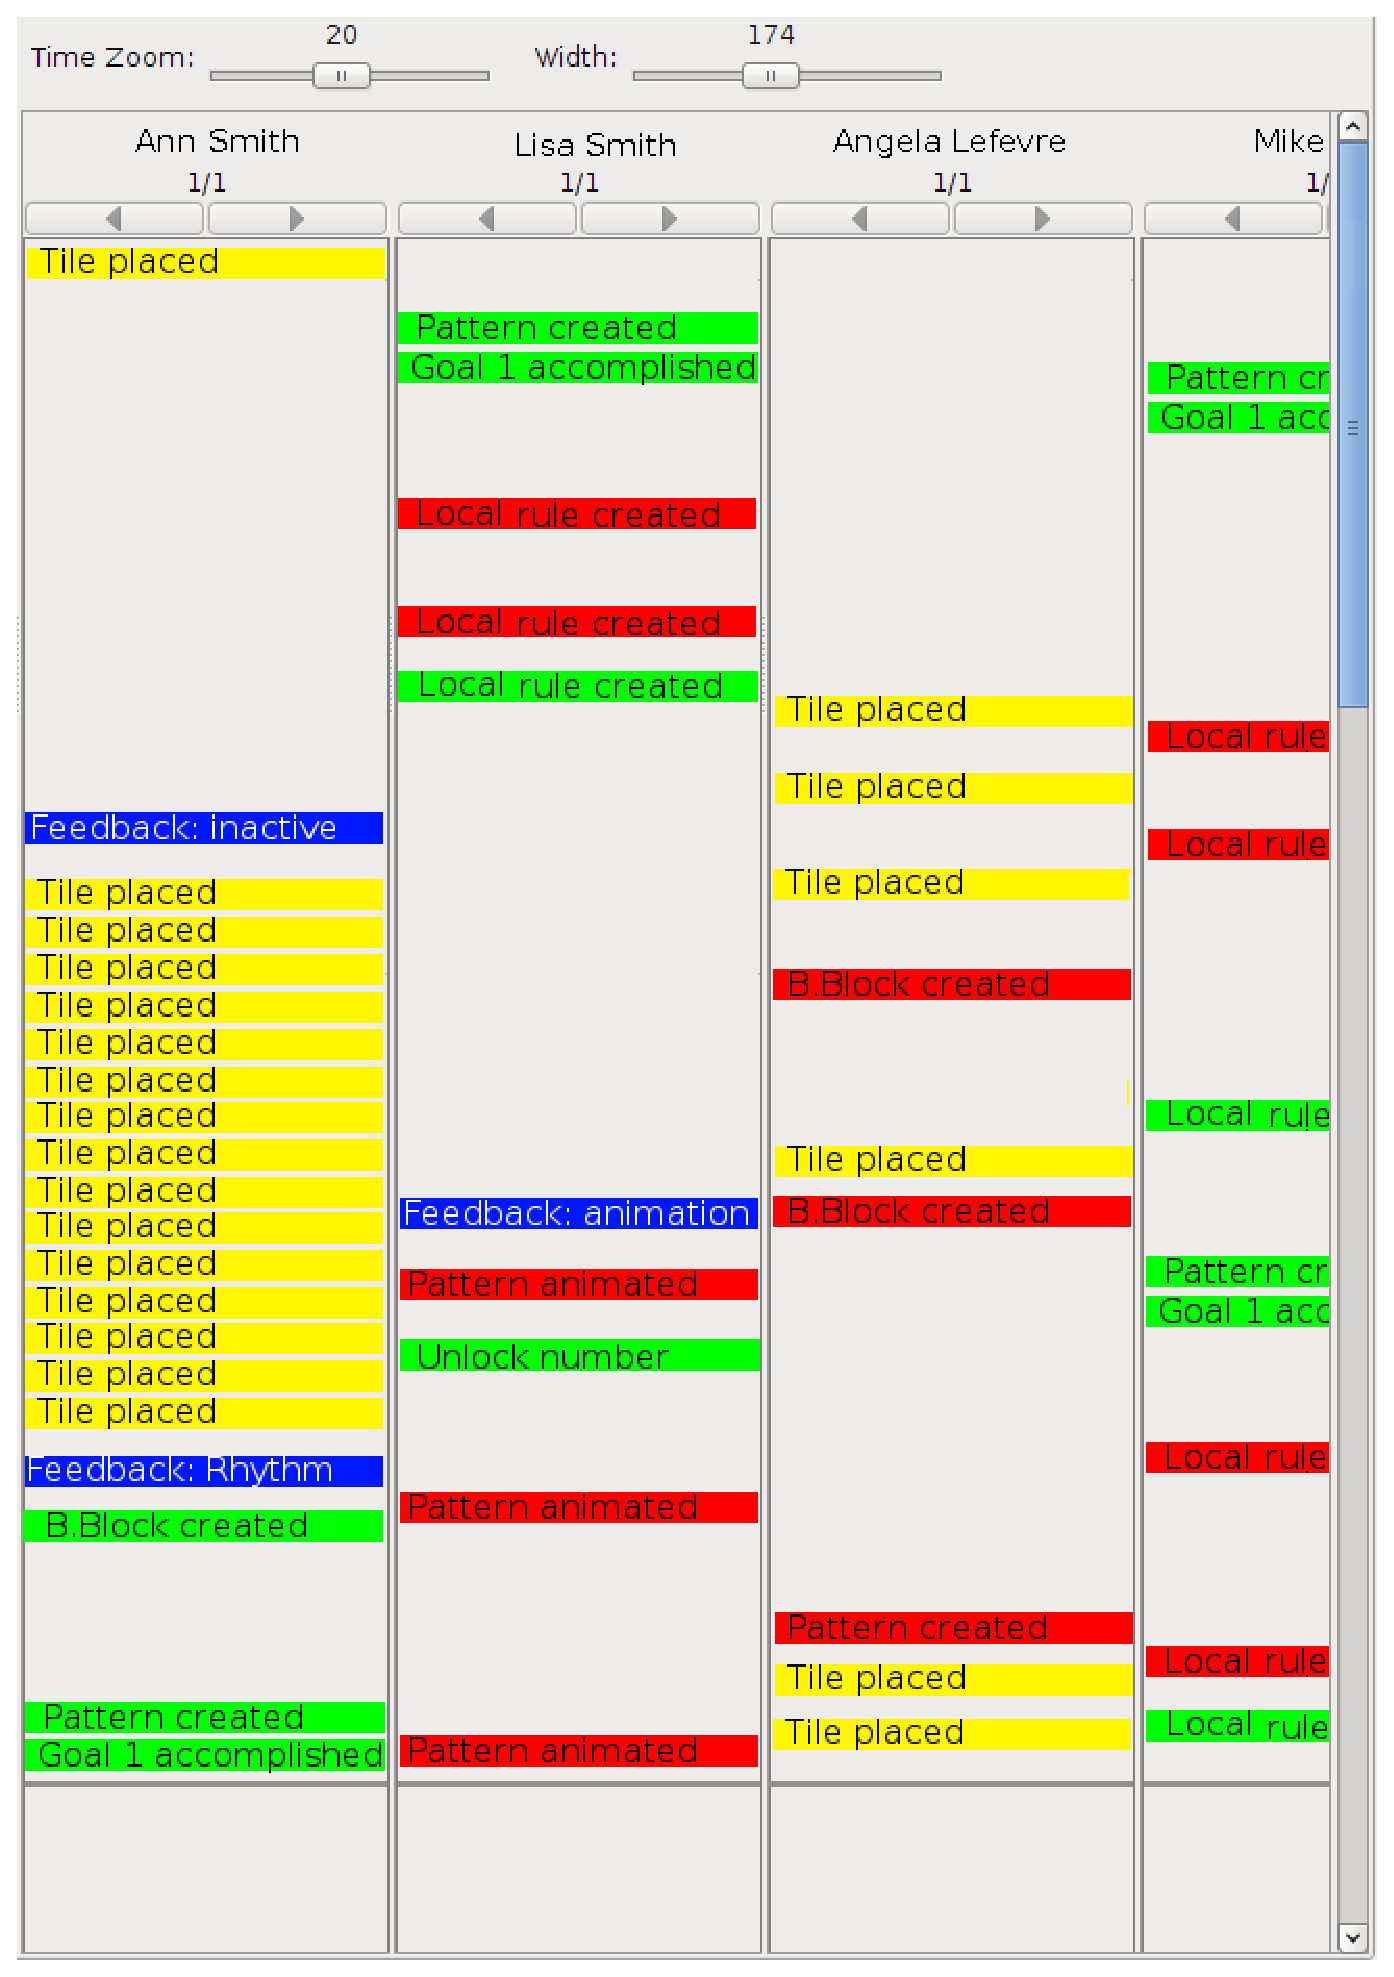
\includegraphics[width=\textwidth]{gfx/ta-st}
  \caption{Student Tracking visualisation, showing the important
    indicators only (i.e. post-Phase C version of the tool)}
  \label{fig:stex}
\end{figure}

\subsection{Classroom Dynamics}
\label{sec:classroom-dynamics}

The CD tool gives the teacher an at-a-glance overview of which
students are currently engaged with the task and who may be in
difficulty and in need of the teacher's help (see Figure 3).  It shows
students as circles on a canvas, showing their initial within the
circle to identify them. The colour of each circle reflects the
student's current activity status as perceived by the system:

\begin{figure}[hbtp]
  \centering
  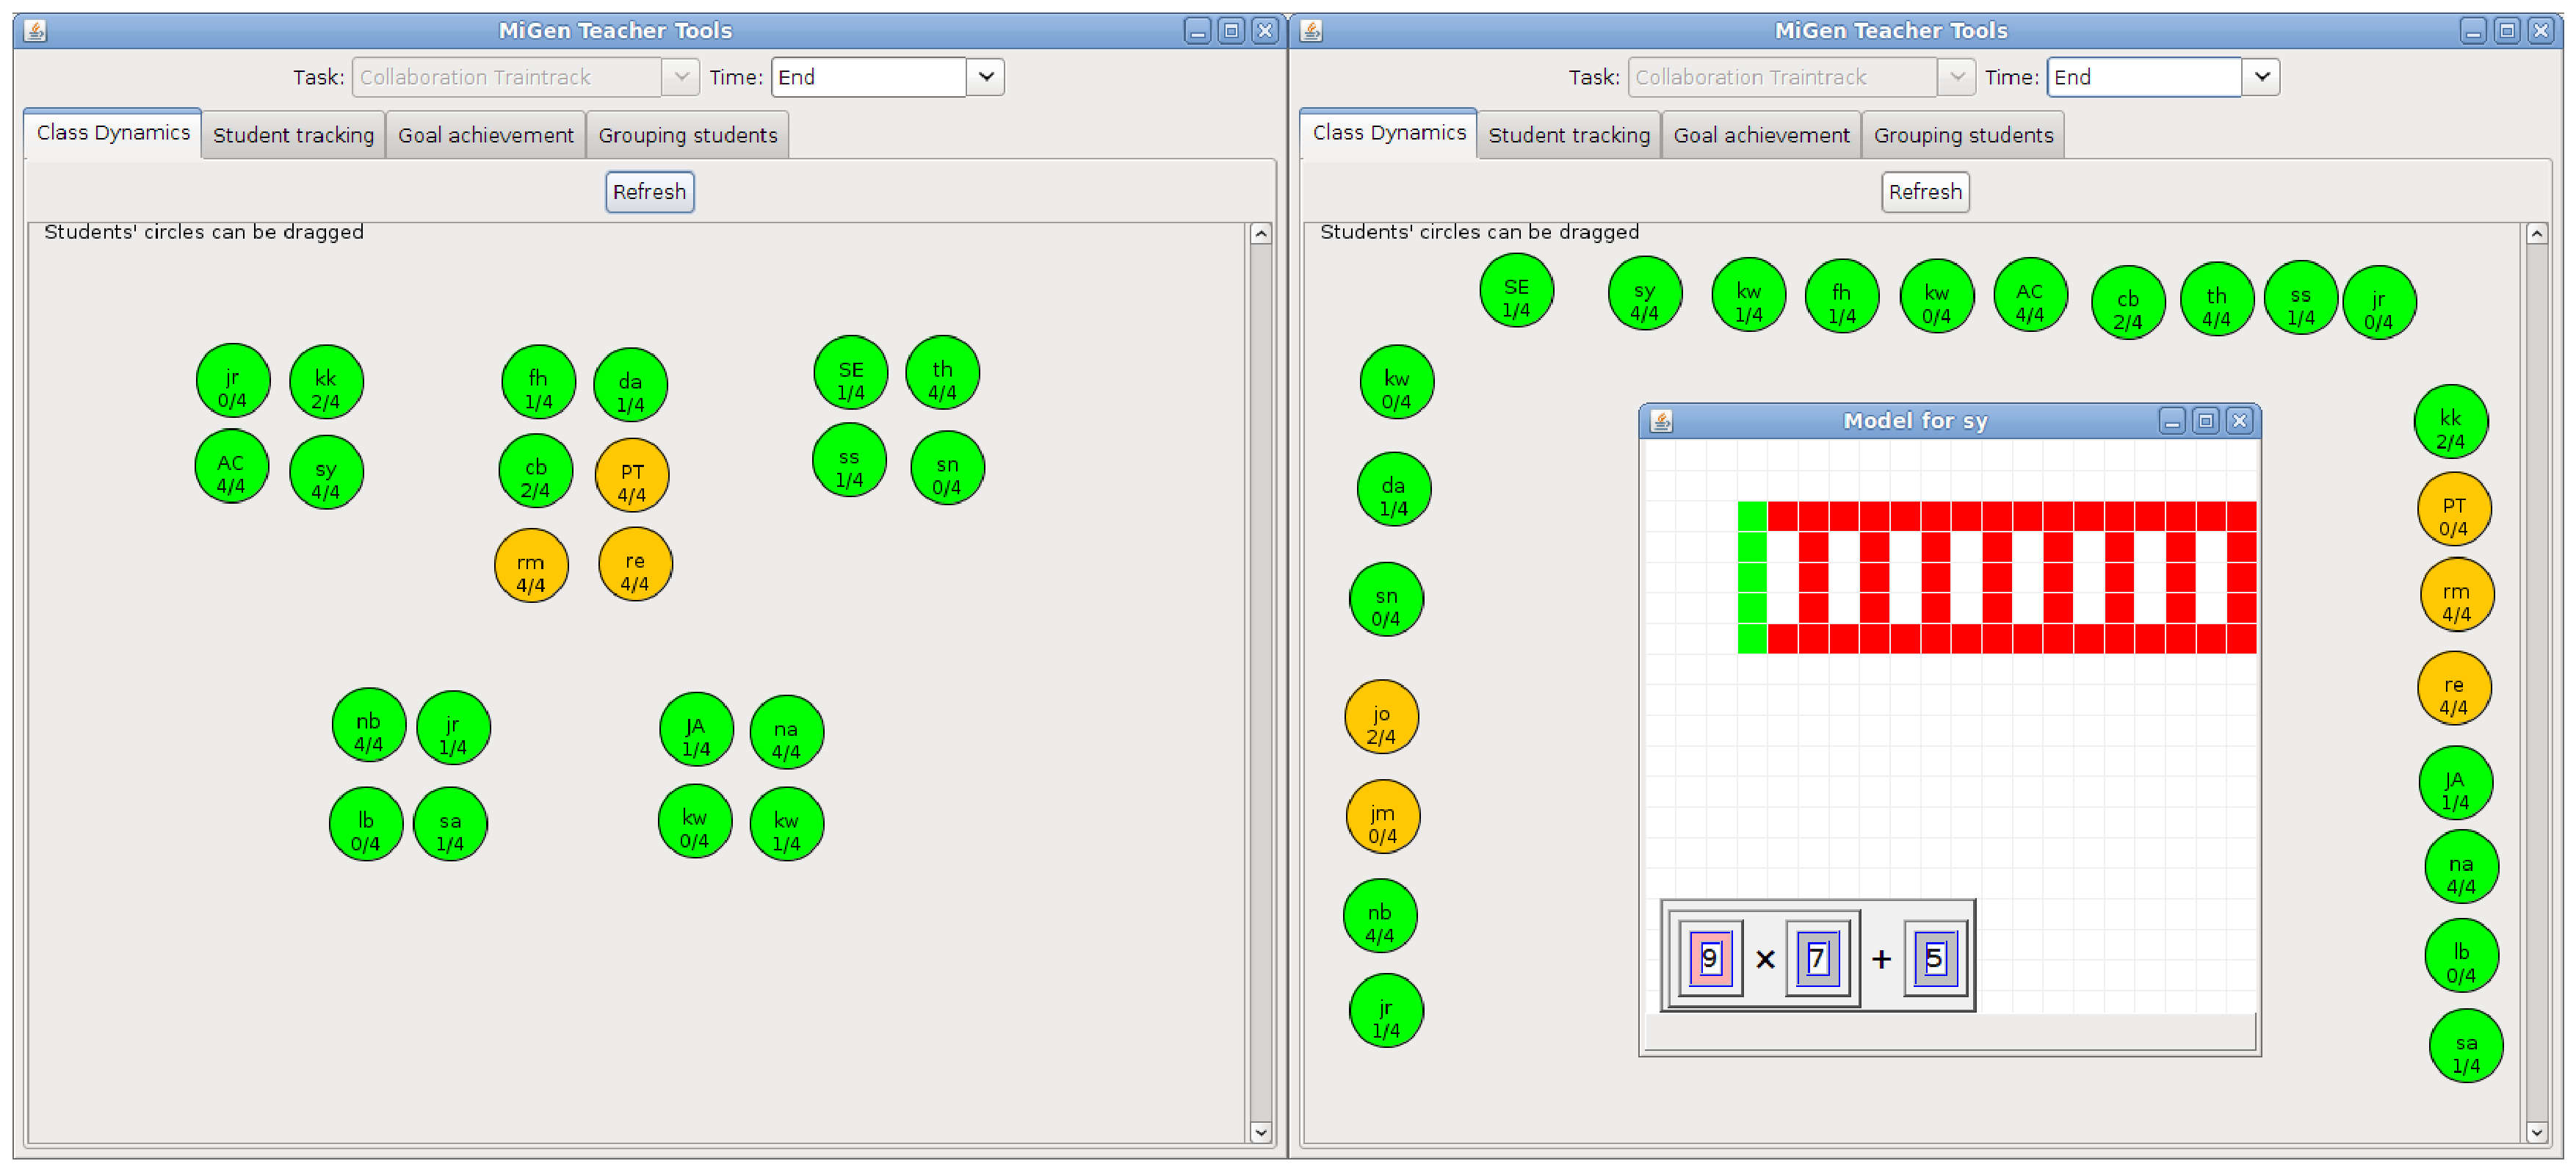
\includegraphics[width=\textwidth]{gfx/ta-cd}
  \caption{Class Dynamics tool}
  \label{fig:ta-cd}
\end{figure}

\begin{itemize}
\item Students shown in Green are active and working constructively on
  the task as far as the system can tell.
\item Students shown in Amber are inactive. This means that they have
  not interacted with the eXpresser for some time (by default, five
  minutes). Unless this is expected by the teacher (for example,
  sometimes teachers interrupt the lesson to address the class and
  explain some common misunderstanding), this usually means that the
  student is distracted, for example talking to fellow student, or
  playing games in their web-browser.
\item Students shown in Red are waiting for the teacher to help
  them. This means that students have requested help from the system
  in a situation where the system’s intelligent support cannot help
  the student any further. At this point, the system displays a
  message “The teacher will come to help you now” and the student’s
  circle becomes coloured Red in the CD tool, to attract the attention
  of the teacher.
\end{itemize}

Hovering over a student´s circle with the cursor shows additional
information about the student: their full name and status: working,
inactive, or waiting for the teacher. The
circles that represent the student can be dragged and moved around on
the canvas. This enables teachers to set up the display so that the
position of the students’ circles on the screen matches the student’s
spatial positioning in the classroom. This helps the teacher to match
what is being displayed in the CD tool with her own observations in
the classroom. It also helps the teacher to identify situations that
may be location-dependent. For example, if several students seated at
the same table show as amber, this might indicate that they are
distracting each other, and that the teacher needs to intervene to
focus their attention on the task again.

An additional optional feature in the CD tool shows the number of
goals achieved so far by the students, as a fraction of the total
number of goals of the task. For example, if a student has achieved
half of the goals of a task which has four goals, this would show 
as~“2/4”. This does not provide information about which task goals have
been achieved, and generally task goals can be achieved in different
orders. In order to provide more detailed information about the
achievement of goals, we developed the Goal Achievement tool.


\subsection{Goal Achievement}
\label{sec:goal-achievement}

The Goal Achievement tool shows detailed information about the
achievement of task goals by students. It allows the teacher to decide
if more explanation is needed for the class as a whole relating to any
of the task goals, if a student who has finished the task can be asked
to help one of the other students, or if the class is ready to move on
to the next task. 

\begin{figure}[hbtp]
  \centering
  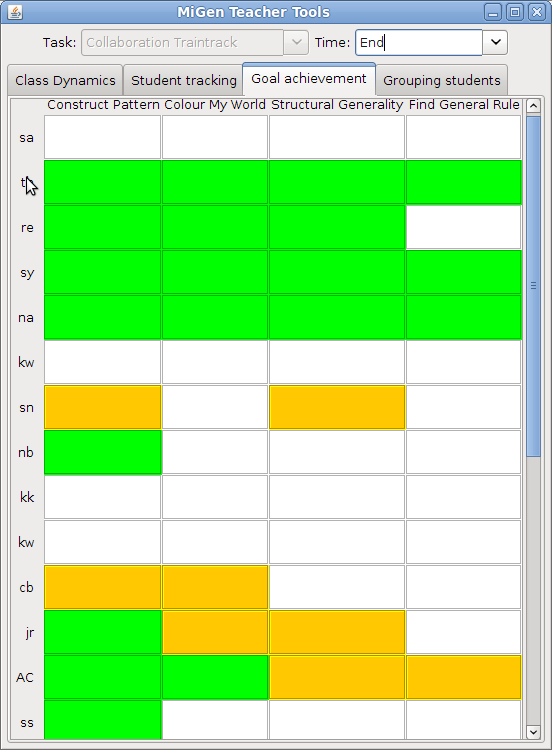
\includegraphics[width=8cm]{gfx/ta-ga}
  \caption{Goal Achievment tool}
  \label{fig:goal-a}
\end{figure}

The GA tool shows a tabular display of students and task goals. Each
row of the table shows the progress of one student (identified by
their initials) in completing the task goals. Each column of the table
shows the completion status of one task goal for all students. The
names of the tasks are shown at the top and the bottom of the
columns. Each student has several cells beside his or her name, one
cell per task goal. Hovering over one of the cells with the cursor
provides the full description of the goal, together with the name of
the student and the achievement status of that goal for that
student. We stress that the goal achievement information inferred by
the eGeneraliser and displayed in the GA tool does not necessarily
correspond to the information about goal achievement that is provided
by the students themselves in their Activity Document: sometimes
students tick as `done’ task goals they believe they have achieved,
but which the system infers have not actually been achieved;
conversely, sometimes students do not tick as `done’ task goals that
the system infers as being achieved.
 
The Goal Achievement tool uses a colour code to identify the current
status of a task goal for each student:

\begin{itemize}
\item A White cell shows that a goal has not been achieved yet by the
student. This is the default status for all cells.
\item A Green cell
shows that the goal is currently being achieved by the student’s
construction.
\item An Amber cell shows that the goal has been achieved
by the student during the course of the current task, but is not being
achieved by the student’s current construction.
\end{itemize}


A task goal can appear as Amber for several reasons. For example, some
students may finish the task much earlier than others. The system
gives such students the opportunity to undertake the task again but
this time following a different construction approach. Such students
would appear with all their task goal cells coloured Amber in the GA
tool and with the cells gradually turning to Green again. Some
students, on the other hand, might not recognise that they have
accomplished a task goal and their further interaction with eXpresser
may result in a situation where the goal is no longer accomplished,
either accidentally (e.g., a pattern was coloured generally but then a
variable is deleted) or in an explicit attempt to achieve some other
task goal (e.g., in order to relate two patterns via the same
variable, the student may have to temporarily leave them
uncoloured). Using three colours for visualising the task goal
achievement information allows the teacher to differentiate between
those students who have moved back and forth taking different
construction approaches to the task and those students who are having
problems completing the task and cannot advance.


\subsection{Time-stop Funcionality}
\label{sec:time-stop-func}

This is a cross-tool functionality provided by all the TA tools. It
allows the user to select a specific point in time, t, with respect to
which the ST, CD and GA visualisations are generated. The tools ignore
all indicator occurrences after that time point, allowing analysis of
the situation at that particular time. In particular, the ST tool
shows the history of indicator occurrences for all students up to time
t, the CD tool shows the current classroom status at time t, and the
GA tool shows the goal achievement information up to time t.  If the
time point selected is in the future, or if no time point is
explicitly selected, the tools show the current situation by default.
 
The time-stop feature has several purposes. Firstly, it allows
teachers to see information relating to a point in time in a past
lesson, in order to understand the context of a particular
situation. For example, using the ST tool after the lesson, the
teacher may detect an unusual situation --- an unexpected sequence of
indicators --- for a student. The teacher can use the CD tool “frozen”
at that particular moment to check what was the status of other
students nearby, e.g. were they all inactive/distracted?
 
Our second motivation was related to the research itself and the fact
that the time-stop functionality allowed the tools to be used by
the research team to explore the students' interaction data arising
from each classroom session.

Our third motivation was enabling the evaluation of the TA tools with
a far larger number of teachers than those who were able to
participate in classroom trials. Being able to use the real data
gathered from the classroom trials and to present that data via the TA
tools, “frozen” at particular moments in the lesson, allowed us to
pose questions to evaluation participants as if they were in the real
classroom at that precise moment. Although the situation is not
identical (the evaluation participants were not under pressure from
students asking for their help or trying to keep the lesson on track
while they used the TA tools), having access to a much larger number
of teachers who could participate in the evaluation of the TA tools
even if they could not trial the TA tools in their own classrooms was
extremely helpful in the design and evaluation of the tools, as
will be discussed below.

\subsection{Example of Use}
\label{sec:example-use}

In order to facilitate readers' understanding of the TA tools, here we 
describe how a typical classroom session may take place. 

The sessions starts. The teacher introduces the lesson for the day,
and instructs students open eXpresser in their computers. Meanwhile
she opens the TA tools in her computer, probably a tablet. For the
first five minutes, students are a bit confused and not focused, and
the teacher mostly walks around the classroom to make them focus on
the task at hand and try to complete the task goals for the day. Once
students are working on their computers, the teacher can take a step
back and use the tools to help her manage the class.

Most of the time, the teacher has the CD tool selected. In a normal
situation, students should appear green (i.e. working). When students
are shown as amber, she knows they are distracted. She can then come
near them to encourage them to work on the task. The CD tool allows
the teacher to detects that students that are engaged with the
computer are not engaged with the learning task at hand: maybe they
are wasting time on a social network or playing a web game. She does
not need to see every screen to check student engagement: the CD tools
does the job.

Some students call the teacher for help raising their hands or by
calling her. The teacher encourages them to get help from the system.
"If the system cannot help you, then I will come to do it", she says,
knowing that students in such a situation will automatically appear
red in the CD tool. Every time a student appears in red, the teacher
comes to the student to help where the system's artificial
intelligence cannot help anymore. If more than one student is shown in
red at the same time, she can click on all students on her tabler to
see at a glance what they have done so far; she can then go first to
the students that is having more difficulties.

Every now and then, the teacher looks at the Goal Achievement tool.
This tool shows the progress of all students on accomplishing the
learning goals for the task. Some students will finish quickly, and
knowing that they have finished the teacher can give them additional
activities for prevent boredom. Other students will advance very
slowly; the teacher can use this information to provide them with
additional homework so that they can learn as much as their peers even
if they need more time than available in the classroom. Sometimes the
tool shows that most students cannot achieve a particular goal; the
teacher can interrupt the class for helping all students at the same
time, maybe clarifying a confusing goal or providing additional
material to help the students' understanding.

At the end of the classroom session, some teachers can use the Student
Tracking tool to examine in detail what some students have done. For
example, if the teacher explained to one student how to relate two
patterns by using the same unlocked number, she can check whether the
student started doing it straight away or required some time of trial
and error to understand the concept.

%%% Local Variables:
%%% mode: latex
%%% TeX-master: "main"
%%% End:
